%!TEX root = ../document.tex
\chapter{Evaluierung} 

	Im Rahmen der Diplomarbeit ist eine Referenzimplementierung entstanden.
	Die Ergebnisse in diesem Kapitel basieren auf Testläufen dieser Referenzimplementierung.

	\section{Testdatensätze}

		Um die Leistung des vorgestellten Verfahrens zu testen wurden folgende Datensätze verwendet. 

		\subsection{Tweet Testdatensätze}

			Aus dem Basisdatensatz von 403222 Tweets wurden zufällig 20000 Datensätze als Testdatensätze gewählt (siehe auch Abschnitt \ref{sub:Datenerhebung}. 
			Diese 20000 werden in den folgenden Abschnitten verwendet.
			Die geografischen Koordinaten der Tweets werden ebenfalls nach dem Verfahren aus Abschnitt \ref{sub:Stadtbestimmen} auf die nächstgelegene Stadt aufgelöst.
			Dieser Schritt wird durchgeführt um einem Tweet eine Verwaltungseinheit erster und zweiter Ordnung sowie ein Land zuzuordnen.
			Zur Bestimmung von Abständen werden weiterhin die ursprünglichen geografischen Koordinaten des Tweets verwendet.  

		\subsection{Testdatensätze für den absoluten und relativen Schwellwert} \label{sub:schwellwerteDatensatz} 

			Um die Qualität der Ergebnisse zu beeinflussen bietet das Verfahren die Möglichkeit individuelle Werte für den Schwellwert der absoluten und relativen Häufigkeiten anzugeben.
			Um das Verfahren zu Testen wurde ein Satz zufällig gewählter Kombinationen für den Schwellwert der absoluten und relativen Häufigkeit erzeugt (siehe Abbildung \ref{img:relHaufBsp}).
			Es wurden 150 verschiedene Kombinationen erstellt.
			Für den Schwellwert der absoluten Häufigkeit wurden Ganzzahlen zwischen den Werten 0 und 110 zufällig gewählt, für den Schwellwert der relativen Häufigkeit wurden Fließkommazahlen zwischen den Werten 0 und 100.
			Dadurch wird es ermöglicht, dass Verfahren mit verschiedenen Werten für die absoluten und relativen Häufigkeiten zu testen.
			Es soll dadurch eine Aussage über den Zusammenhang zwischen den Schwellwerten und der Qualität der Ergebnisse des Verfahrens zur Geolokalisierung getroffen werden.


			In Abbildung \ref{img:random2d} sind die erzeugten Kombinationen aufgetragen.

			\begin{figure}[!ht]
				\centering
				\makebox[\textwidth]{
				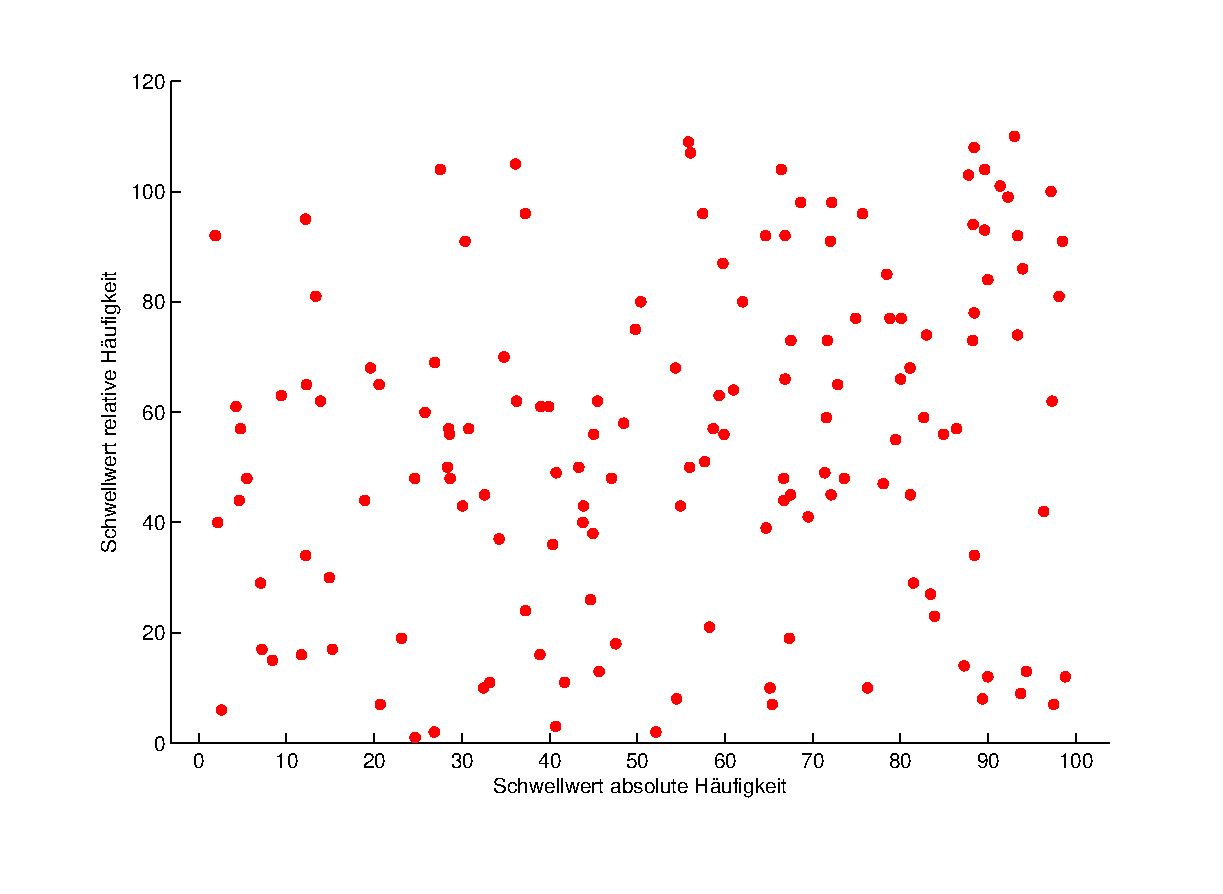
\includegraphics[scale=0.8]{matlabPlot/rand2D.eps} 
				} 
				\caption{Testdatensätze für die Schwellwerte}
				\label{img:relHaufBsp}
			\end{figure}

	\section{Kennzahlen zur Messung der Qualität} \label{sec:Kennzahlen} 

		Es werden nun einige Kennzahlen zur Messung der Qualität der Ergebnisse eingeführt.
		Diese werden anhand der untersuchten Hierarchieebene unterteilt.
		Die Städteebene, also die unterste Hierarchieebene, wird dabei anders behandelt als die restlichen Hierarchieebenen.

		Auf der untersten Ebene werden Fehlerdistanzen verwendet.
		Diese geben an wie weit die tatsächliche geografische Position, von der ein Tweet versendet wurde, von der durch die Geolokalisierung zugeordneten geografischen Position (die geografischen Koordinaten der Stadt) entfernt ist.
		Dies lässt eine Detailanalyse der Ergebnisse zu.

		Auf den höheren Ebenen, die eine größere geografische Region beschreiben, ist dies allerdings nicht sinnvoll.
		Ein große geografische Region kann nicht durch einen einzelnen Punkt beschrieben werden. 
		Es wird deshalb nur entschieden ob die Geolokalisierung dem untersuchten Tweet die korrekte geografische Region zuordnet. 
		Einfach ausgedrückt: Ist der Tweet tatsächlich aus der geografischen Region abgesendet worden die ihm durch die Geolokalisierung zugeordnet wurde?
		Es werden also Treffer und Nicht-Treffer gegenübergestellt. 
		
		\subsection{Kennzahlen zur Qualitätsbewertung auf Städteebene}

			Als Grundlage zur Bewertung auf Städteebene werden Fehlerdistanzen verwendet.

			$p^f_{i}$ gibt die geografische Position eines Tweets $i$ an, welche durch die Geolokalisierung bestimmt wurde.
			$p^r_{i}$ gibt die reale geografische Position des Tweets $i$ an. 
			Die Funktion $dist(u,v)$ gibt die Distanz zwischen geografischen Positionen $u$ und $v$ an.

			\subsubsection{Ergebnismenge}

				Unter der Ergebnismenge wird die Anzahl derjenigen Tweets aus den Testdatensätzen verstanden, denen durch die Geolokalisierung eine Georeferenz zugeordnet werden konnte.
				Dabei wird die Korrektheit der zugeordneten Georeferenz nicht berücksichtigt.
				Die Ergebnismenge wird in den Formeln mit $|erg|$

			\subsubsection{Durchschnittliche Fehlerdistanz} 

				Dabei wird die Summe der Fehlerdistanzen durch die Ergebnismenge geteilt.
				Die durchschnittliche Fehlerdistanz $p_{avg}$ errechnet sich durch die Formel:

				\begin{equation}
					p_{avg}=\frac{\sum_{i=0}^{|erg|}{dist(p^f_i,p^r_i)}}{|erg|}
				\end{equation}	

				Umso kleiner die durchschnittliche Fehlerdistanz ist, umso besser ist das Ergebnis.

			\subsubsection{Median der Fehlerdistanz}

				Zur Bewertung der Distanzen wird neben der durchschnittlichen Fehlerdistanz der Median der Fehlerdistanz betrachtet.
				Durch diesen Wert können die Ergebnisse noch genauer untersucht werden. 
				Im Gegensatz zur durchschnittlichen Fehlerdistanz ist der Median robust gegenüber Ausreissern.

				Umso kleiner die Median Fehlerdistanz ist, umso besser ist das Ergebnis.

		\subsection{Kennzahlen zur Qualitätsbewertung der Verwaltungseinheiten erster und zweiter Ordnung sowie Länderebene} 

			Die Verwaltungseinheit erster Ordnung, die Verwaltungseinheit zweiter Ordnung und die Länder bestehen aus größeren geografischen Regionen.
			Es soll nun nur noch betrachtet werden ob die tatsächliche geografische Region eines Tweets mit derjenigen übereinstimmt die durch die Geolokalisierung bestimmt wurde.
			
			\subsubsection{True Positive (TP)}

				Dieser Wert gibt an wie viele der Tweets durch die Geolokalisierung der korrekten geografischen Region zugeordnet werden konnten.
				
			\subsubsection{False Positive (FP)}

				Gibt an wie viele der Tweets der falschen geografischen Region zugeordnet wurden.  

			\subsubsection{Precision}  

				Beschreibt den Anteil der Ergebnismenge, der durch die Geolokalisierung korrekt zugeordnet wurde.
				Der Optimalwert liegt bei 1,0.
				Dieser lässt sich wie folgt berechnen:

				\begin{equation}
					precision=\frac{TP}{|erg|}
				\end{equation}	

				Die Ergebnismenge entspricht hier der Summe aus TP und FP.
				Womit sich die Formel auch folgendermaßen definieren lässt:  

				\begin{equation}
					precision=\frac{TP}{TP+FP}
				\end{equation}		

			\subsubsection{Recall} 

				Der Recall gibt an welchem Anteil an der Gesamtmenge der getesteten Tweets durch die Geolokalisierung eine korrekte Georeferenz zugeordnet wurde.
				Auch beim Recall liegt der Optimalwert bei 1,0.
				Der Recall lässt sich berechnen durch:

				\begin{equation}
					recall=\frac{TP}{|getestete Tweets|}
				\end{equation}	


				Dieser Wert kann auch folgendermaßen interpretiert werden:
				Der Recall, gibt die Wahrscheinlichkeit an, dass ein zufällig gewählter Tweet, korrekt lokalisiert wird. 

		\subsection{Trade-Off}

			In der Ökonomie bedeutet der Trade-Off die gegenläufige Abhängigkeit von Kosten und Qualität.
			Es müssen Kosten in Kauf genommen werden um die Qualität zu verbessern. \footnote{Vergleiche http://de.wikipedia.org/wiki/Trade-off\#.C3.96konomie} 
			
			Bei den vorliegenden Ergebnissen kann der Median oder die Precision als Qualität interpretiert werden.
			Die Ergebnismenge oder der Recall können als Kosten betrachtet werden.
			Welche der Kennzahlen die Qualität darstellt und welcher die Kosten kommt auf die jeweiligen Anforderungen an. 

			Im Kern geht es darum, dass jeweils einer der beiden Werte auf Kosten des anderen optimiert werden kann.
			Durch die Optimierung des Trade-Off wird eine Kombination gefunden, welche das Optimum zwischen Kosten und Qualität darstellt.

			In allen Hierarchieebenen wird zusätzlich ein Optimum für den Trade-Off berechnet. 

			Auf Städteebene wird der Median in Kombination mit der Ergebnismenge betrachtet oder die durchschnittliche Fehlerdistanz in Kombination mit der Ergebnismenge.
			Auf den anderen Hierarchieebenen wird die Precision in Kombination mit dem Recall betrachtet.

	\section{Ergebnisse}

		Die Kennwerte für die Hierarchieebenen wurden bestimmt indem für jede Kombination aus Schwellwerten alle 20000 Tweets des Testdatensatzes untersucht wurden.
		Für vier geografische Hierarchieebenen wurden 150 verschiedene Kombinationen von Schwellwerten auf jeweils 20000 Tweets getestet.
		Dies entspricht $4*150*20000 = 12000000$ Durchläufen der Geolokalisierung.

		Es werden hier nun die Ergebnisse der Testläufe vorgestellt und analysiert.
		Zunächst werden die optimalen Werte für die einzelnen Hierarchieebenen und deren Kennzahlen betrachtet.


		\subsection{Vergleich der Ergebnisse mit unterschiedliche Schwellwerten} 

			Es werden hier die Ergebnisse aller Durchläufe betrachtet.
			Dabei werden die Kennzahlen aus Abschnitt \ref{sec:Kennzahlen} pro getestetem Schwellwerte aufgetragen. 
			Es werden dadurch mögliche Zusammenhang zwischen den gewählten Schwellwerten und den Ergebnissen abgeleitet.
			Eines der Ziele dieser Arbeit bestand darin das Verfahren bezüglich der Qualität der Ergebnisse justierbar zu machen.
			Dies wird über die Schwellwerte realisiert.
			Es wird jede der vier Hierarchieebenen einzeln bewertet um zu verifizieren, dass die Angabe der Schwellwerte zur Justierung auf jeder Hierarchieebene verwendet werden kann.

			\subsubsection{Ergebnisse zur Stadtebene}

				Auf der Stadtebene wird die Median Fehlerdistanz (siehe Abbildung \ref{img:medianF}) und die durchschnittliche Fehlerdistanz (siehe Abbildung \ref{img:durchschnF}) betrachtet.

				Bei gleichbleibendem Wert für die absolute Häufigkeit zieht eine Änderung des Schwellwertes der relativen Häufigkeit eine Änderung der Kennzahlen nach sich. 
				Wohingegen bei gleichbleibendem Wert für die relative Häufigkeit und einer Änderung der absoluten Häufigkeit kaum eine Änderung der Kennzahlen zu verzeichnen ist.

				Der Schwellwert für die relative Häufigkeit kann zur Justierung der Median Fehlerdistanz und der durchschnittlichen Fehlerdistanz genutzt werden.
				Gegenüber Änderungen des absoluten Schwellwertes verhält sich das Verfahren gleichbleibend bezüglich der Kennzahlen auf Stadtebene.
				Umso kleiner der Schwellwert für die relative Häufigkeit gewählt wird um so kleiner wird der Wert der beiden Kennzahlen.

				In Abbildung \ref{img:citiesRecall} ist die Ergebnismenge aufgetragen.
				Der Schwellwert für die absolute Häufigkeit hat bei gleichbleibender relativer Häufigkeit wiederum nur einen geringen Einfluss auf die Ergebnisse. 

				Niedrige Werte für die relative Häufigkeit erhöhen die Ergebnismenge.
				Die Kennzahlen der Fehlerdistanz verhalten sich also konträr zum Wert der Ergebnismenge.
				Geringere Ergebnismengen verbessern die Fehlerdistanzen(geringere Fehlerdistanzen) und die Qualität nimmt zu.		

				In Tabelle \ref{tab:optCity} sind die besten Werte für die Kennzahlen auf Städteebene zusammengestellt. 
				In den Zeilen 1-3 ist der jeweils beste ermittelte Wert fett gedruckt.
				
				In Zeile 1 ist der beste Wert der Ergebnismenge dargestellt.
				Dieser liegt bei 15819, das bedeutet es konnten 15819 Tweets, und damit 79,1\% der untersuchten Tweets eine Stadt zugeordnet werden.
				Der Wert des Median gibt an, dass 50\% dieser Tweets im Umkreis von 20,43km um die die zugeordnete Stadt versendet wurden.
				Im Durchschnitt weißen alle 15819 Tweets eine Fehlerdistanz von 1423km auf.

				Zeile 4 ist der beste Trade-Off der ermittelt wurde.
				Für den Trade-Off liegt die Ergebnismenge bei 10642(53,21\%).
				50\% dieser Tweets (ca. 25\% aller untersuchter Tweets) denen eine Stadt zugeordnet werden konnte liegen im Umkreis von 9,17km zu der jeweils zugeordneten Stadt.
				Die durchschnittliche Fehlerdistanz reduziert sich gegenüber Zeile 1 auf 548,98km. 

				In Zeile 3 ist der beste Wert der durchschnittlichen Fehlerdistanz angegeben, dieser entspricht 5,53km.
				Die Ergebnismenge liegt jedoch bei 16(0,08\%).

				\begin{table}[h]
					\centering
					\begin{tabular}{|l|r|r|r|r|r|}
					\hline
					  & \multicolumn{1}{c|}{\begin{tabular}[c]{@{}c@{}}Schwellwert\\ relativ\end{tabular}} & \multicolumn{1}{c|}{\begin{tabular}[c]{@{}c@{}}Schwellwert\\ absolut\end{tabular}} & \multicolumn{1}{c|}{\begin{tabular}[c]{@{}c@{}}Ergebnismenge\\ (Anteil)\end{tabular}} & \multicolumn{1}{c|}{\begin{tabular}[c]{@{}c@{}}Median\\ Fehlerdist.\end{tabular}} & \multicolumn{1}{c|}{\begin{tabular}[c]{@{}c@{}}Durchschn.\\ Fehlerdis.\end{tabular}} \\ \hline
					1 & 2.59                                                                               & 6                                                                                  & \textbf{15819(79.1\%)}                                                                 & 20432.24                                                                          & 1423698.12                                                                           \\ \hline
					2 & 97,48                                                                              & 7                                                                                  & 198(0.99\%)                                                                         & \textbf{3242.66}                                                                  & 188573.42                                                                            \\ \hline
					3 & 91.37                                                                              & 101                                                                                & 16(0.08\%)                                                                             & 6016.68                                                                           & \textbf{5532.02}                                                                     \\ \hline \hline
					4 & 26.84                                                                              & 2                                                                                  & \textbf{10642(53.21\%)}                                                                         & \textbf{9168.98}                                                                  & 548979.19                                                                            \\ \hline
					\end{tabular}
					\caption{Zusammenfassung der besten Ergebnisse auf Stadtebene}
					\label{tab:optCity}
					\end{table}

				\begin{figure}[H]
					\centering
					\makebox[\textwidth]{
					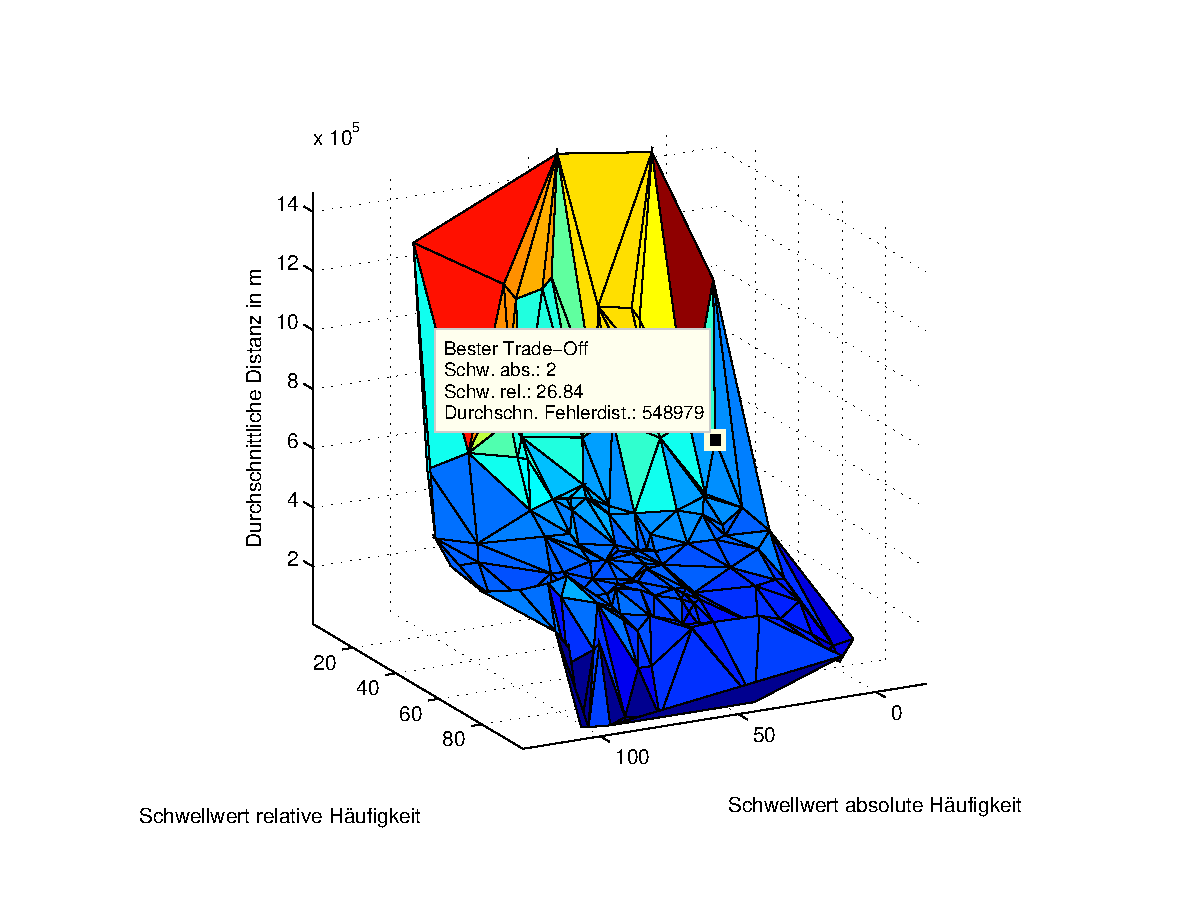
\includegraphics[scale=0.5]{matlabPlot/citiesAVG.eps} 
					} 
					\caption{Durchschnittliche Fehlerdistanz}
					\label{img:durchschnF}
				\end{figure}


				\begin{figure}[H]
					\centering
					\makebox[\textwidth]{
					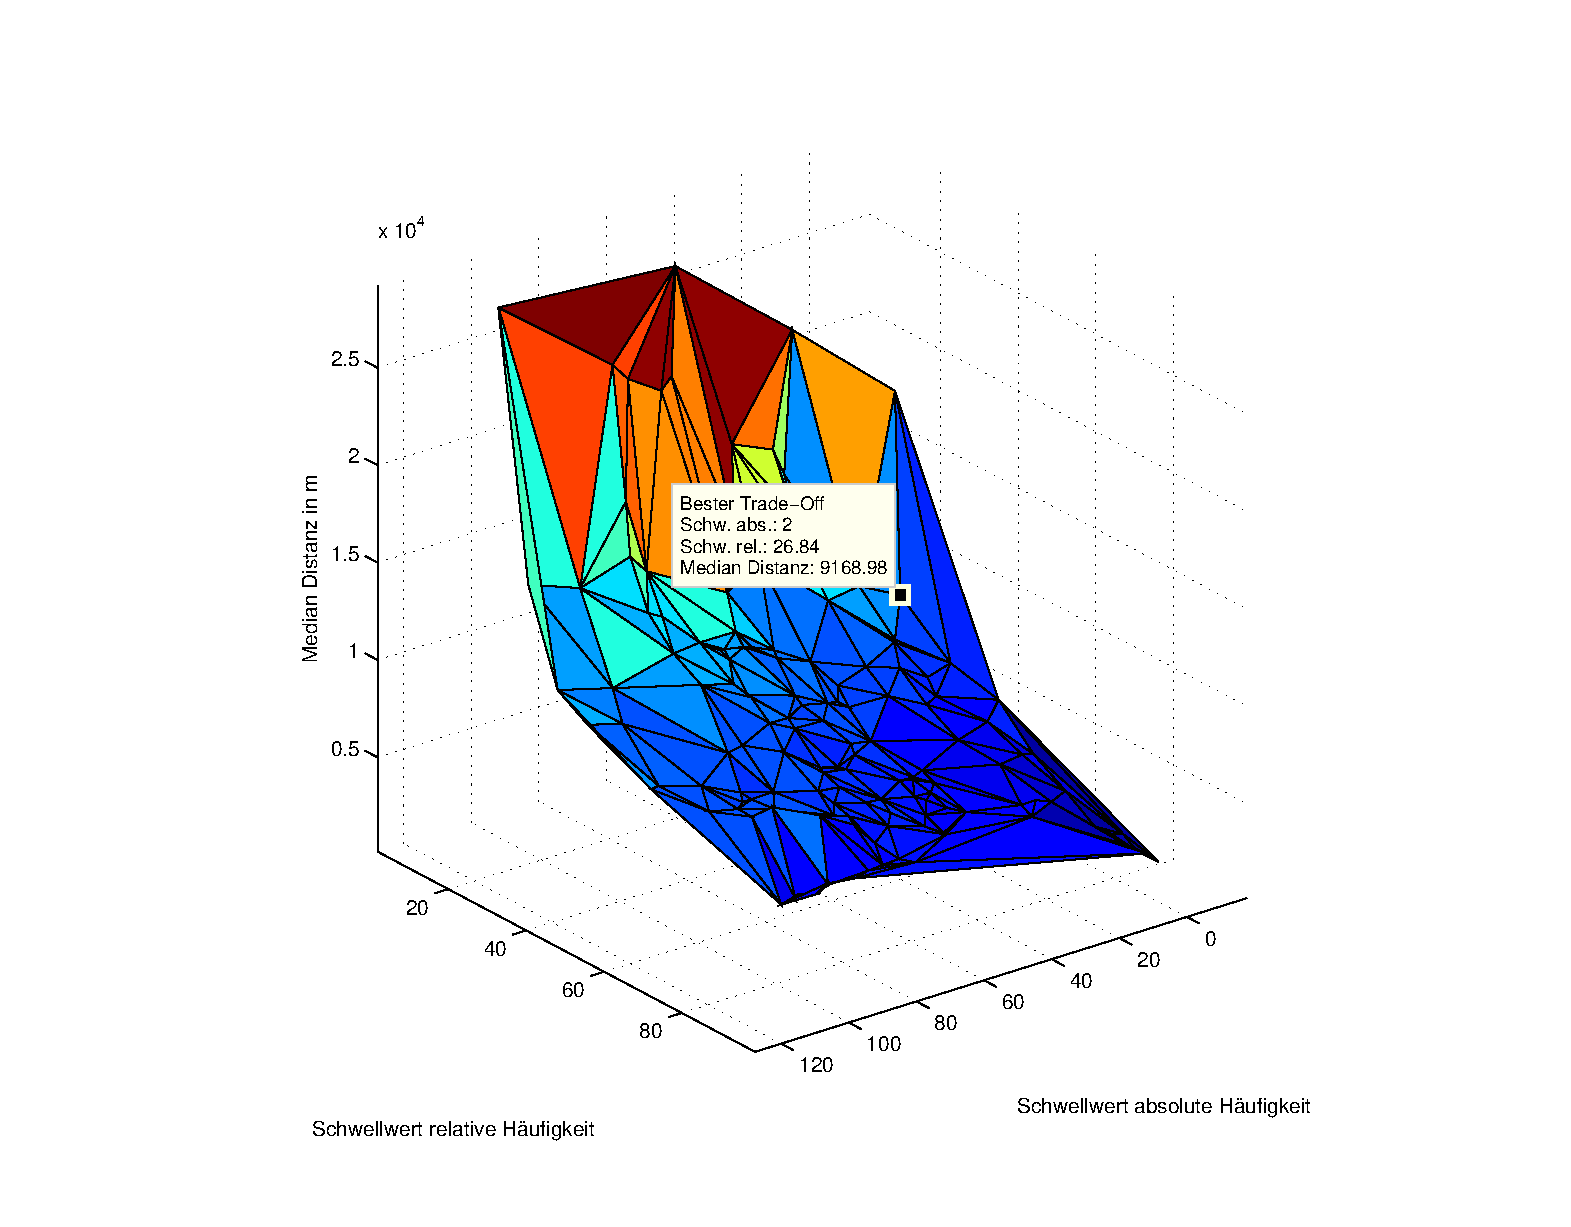
\includegraphics[scale=0.4]{matlabPlot/citiesMedian.eps} 
					} 
					\caption{Median Fehlerdistanz}
					\label{img:medianF}
				\end{figure}



				\begin{figure}[H]
					\centering
					\makebox[\textwidth]{
					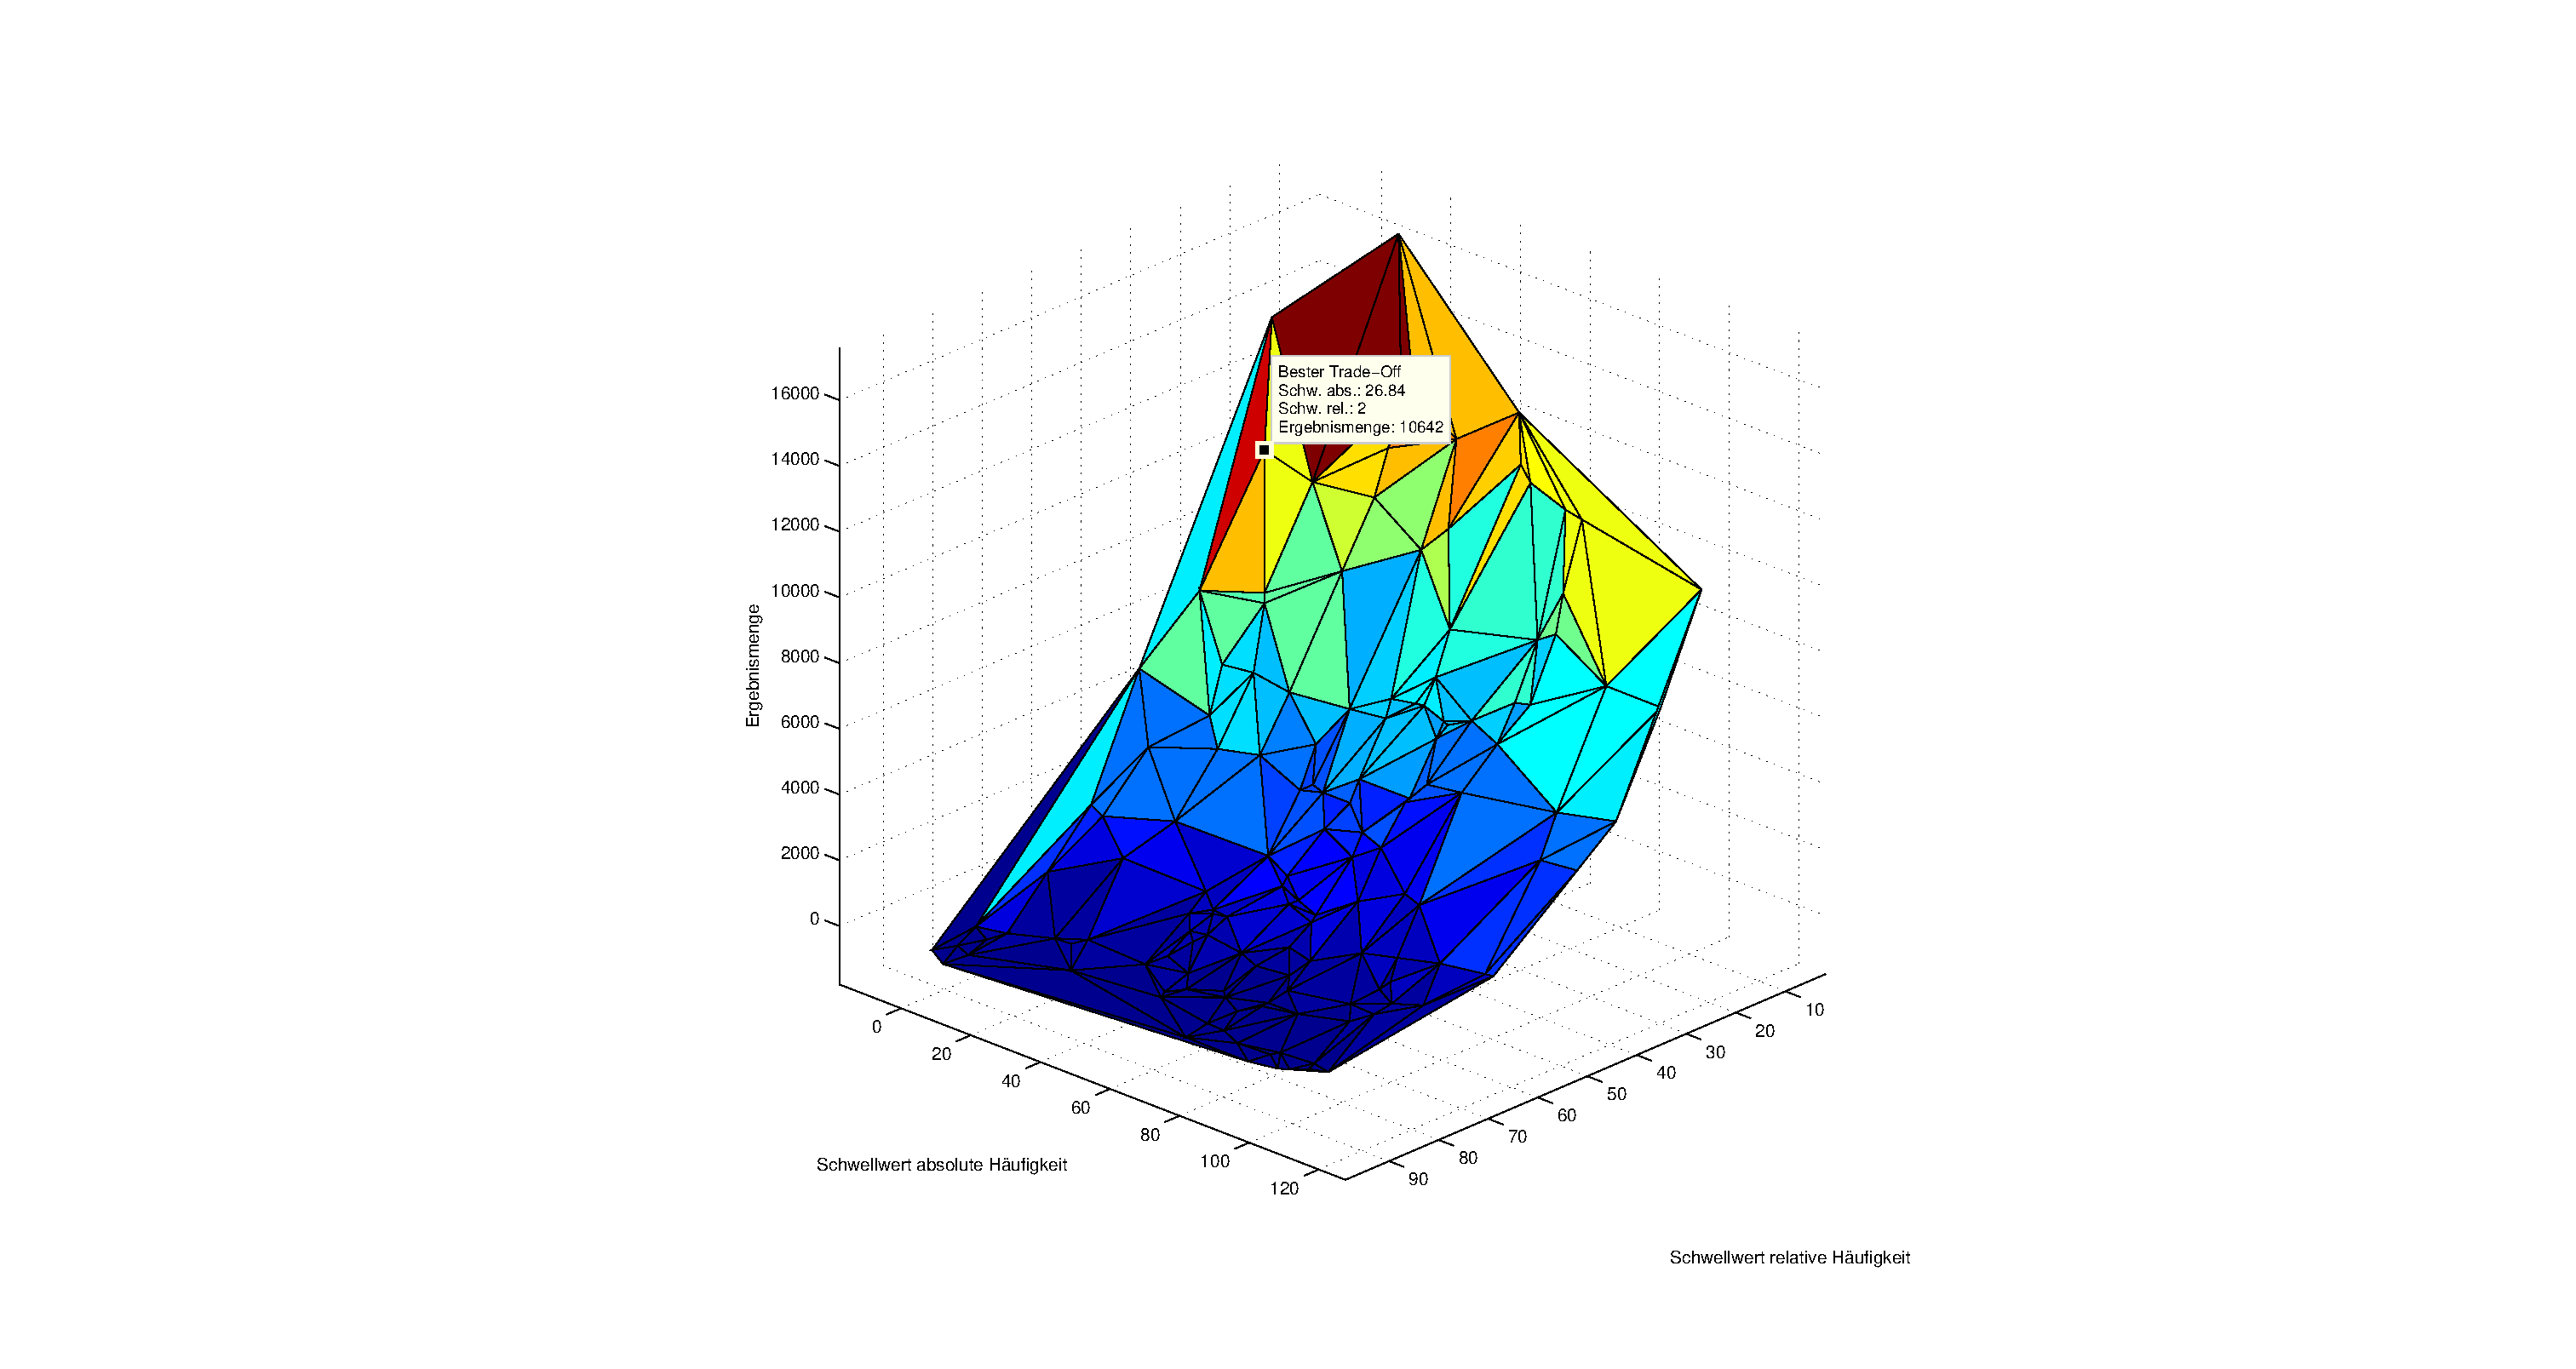
\includegraphics[scale=0.3]{matlabPlot/citiesRecallNEW.eps} 
					} 
					\caption{Ergebnismenge}
					\label{img:citiesRecall}
				\end{figure}

			\subsubsection{Ergebnisse zur Verwaltungseinheit erster und zweiter Ordnung, Land}

				Als Kennzahlen werden nun Precision und Recall herangezogen. 
				In Abbildung \ref{img:precAll} sind die Werte der Precision für die Verwaltungseinheit erster(Adm1) und zweiter Ordnung(Adm2) sowie Land aufgetragen.

				Wie auf Stadtebene auch, beeinflusst hier lediglich der Schwellwert für die relative Häufigkeit das Ergebnis für die Precision. 
				Eine höherer Wert für den Schwellwert der relativen Häufigkeit verbessert den Wert Precision.
				Eine Änderung des Schwellwertes für die absolute Häufigkeit hat bei gleichbleibendem Wert für die relative Häufigkeit kaum einen Einfluss auf den Wert der Precision.
				Dies gilt für alle Hierarchieebenen wie in den drei Plots in Abbildung \ref{img:precAll} zu erkennen ist. 

				Vergleicht man die Plots in Abbildung \ref{img:adm2Recall} so weißen auch diese dieselbe Charakteristik. 
				Im Gegensatz zur Precision hat der Schwellwert für die absolute Häufigkeit einen Einfluss auf den Recallwert.
				Bei gleichbleibendem Schwellwert für die relative Häufigkeit, kann durch die Absenkung des Schwellwertes der absoluten Häufigkeit eine Verbesserung des Recall erreicht werden.
				Da der Wert der absoluten Häufigkeit keinen Einfluss auf die Precision hat kann dieser erhöht werden um das Ergebnis zu optimieren.

				Wiederum beeinflusst der Schwellwert für die relative Häufgikeit die Qualität konträr.
				Umso größer der Schwellwert der relativen Häufigkeit gewählt wird umso schlechter wird der Recallwert, gleichzeitig verbessert sich allerdings die Precision.

				Ein vorgehen bei der Wahl der Schwellwerte ist es eine gewünschte Precision zu wählen und danach den Schwellwert der realtiven Häufigkeit zu bestimmen.
				Danach kann der Schwellwert der absoluten Häufigkeit zur Optimierung des Recall minimiert werden. 			

				\begin{figure}[htb]
				\centering
				  \begin{tabular}{@{}ccc@{}}
				    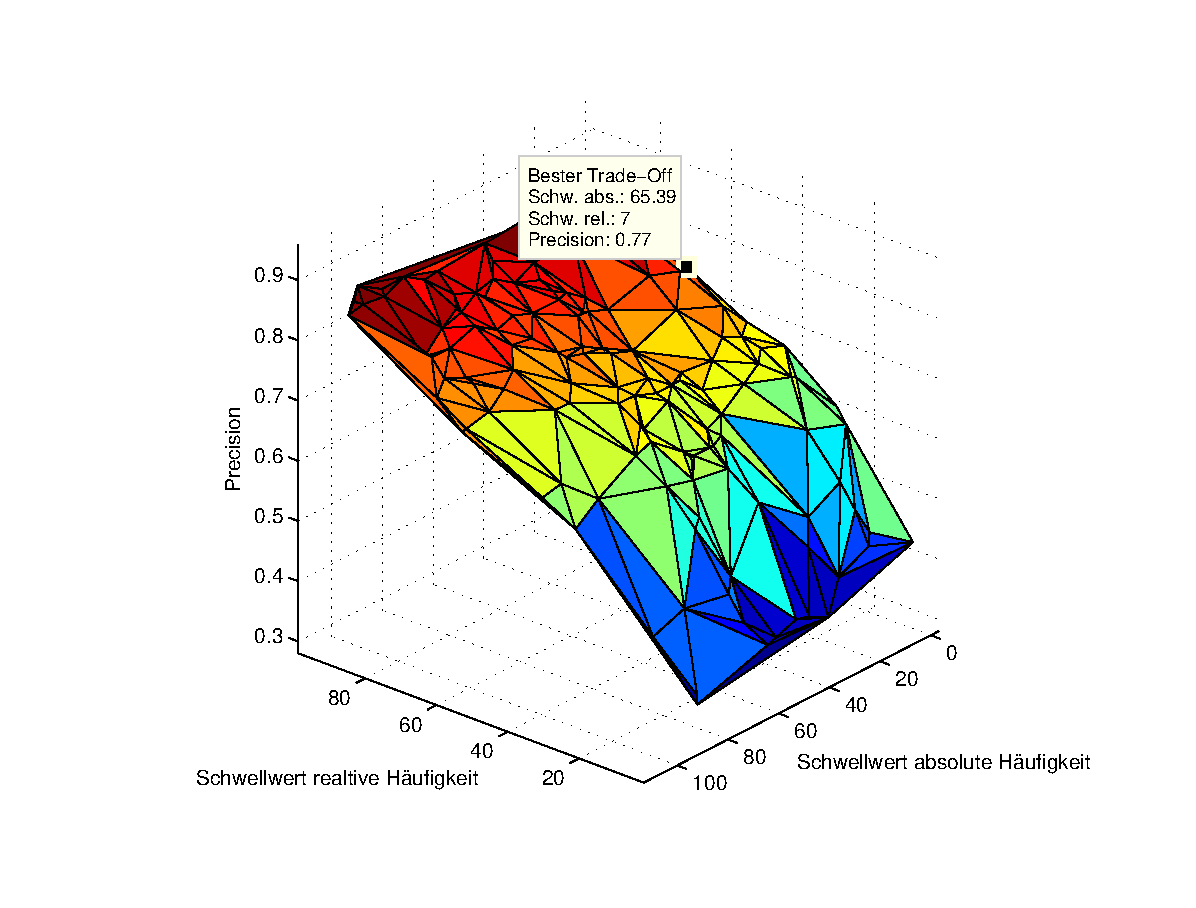
\includegraphics[width=.5\textwidth]{matlabPlot/adm2Prec.eps}  &
				   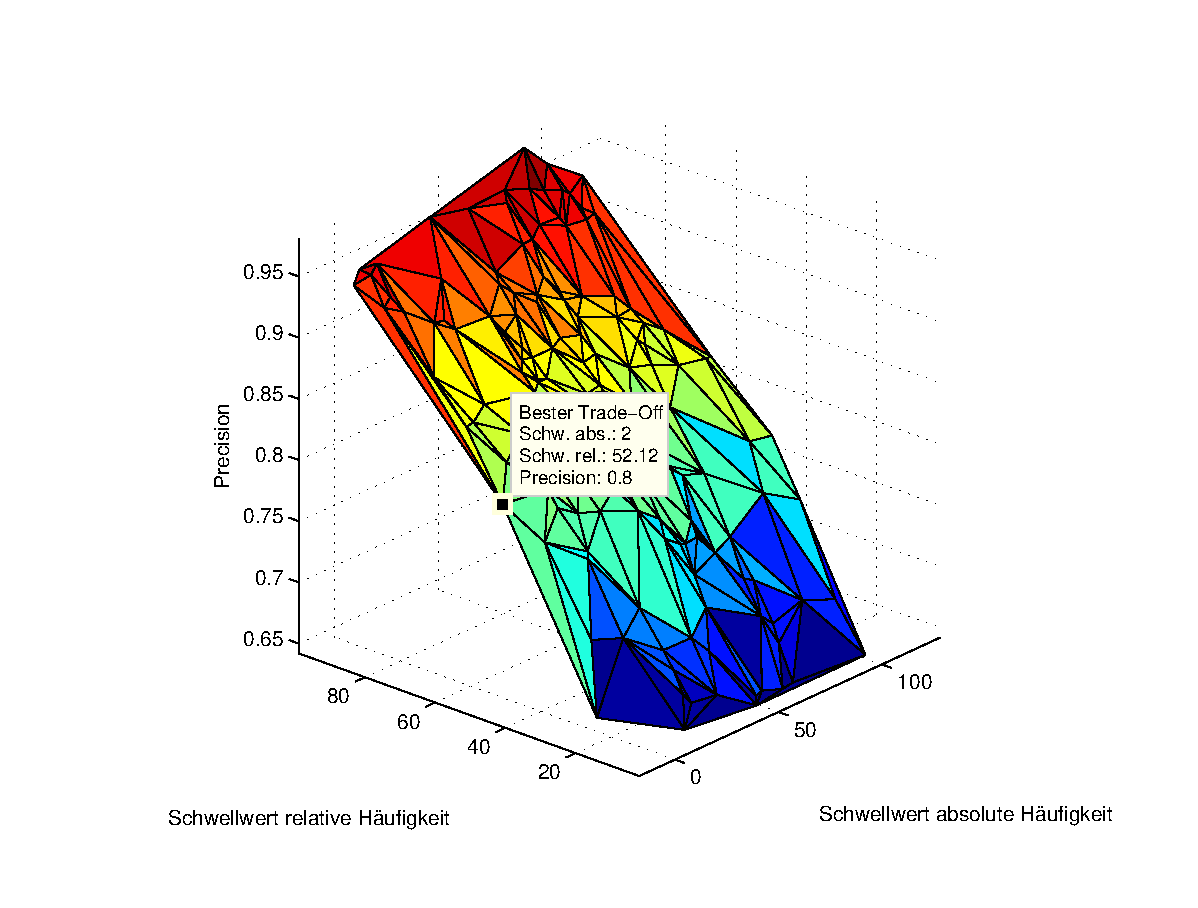
\includegraphics[width=.5\textwidth]{matlabPlot/adm1Prec.eps}	\\
				   \multicolumn{2}{c}{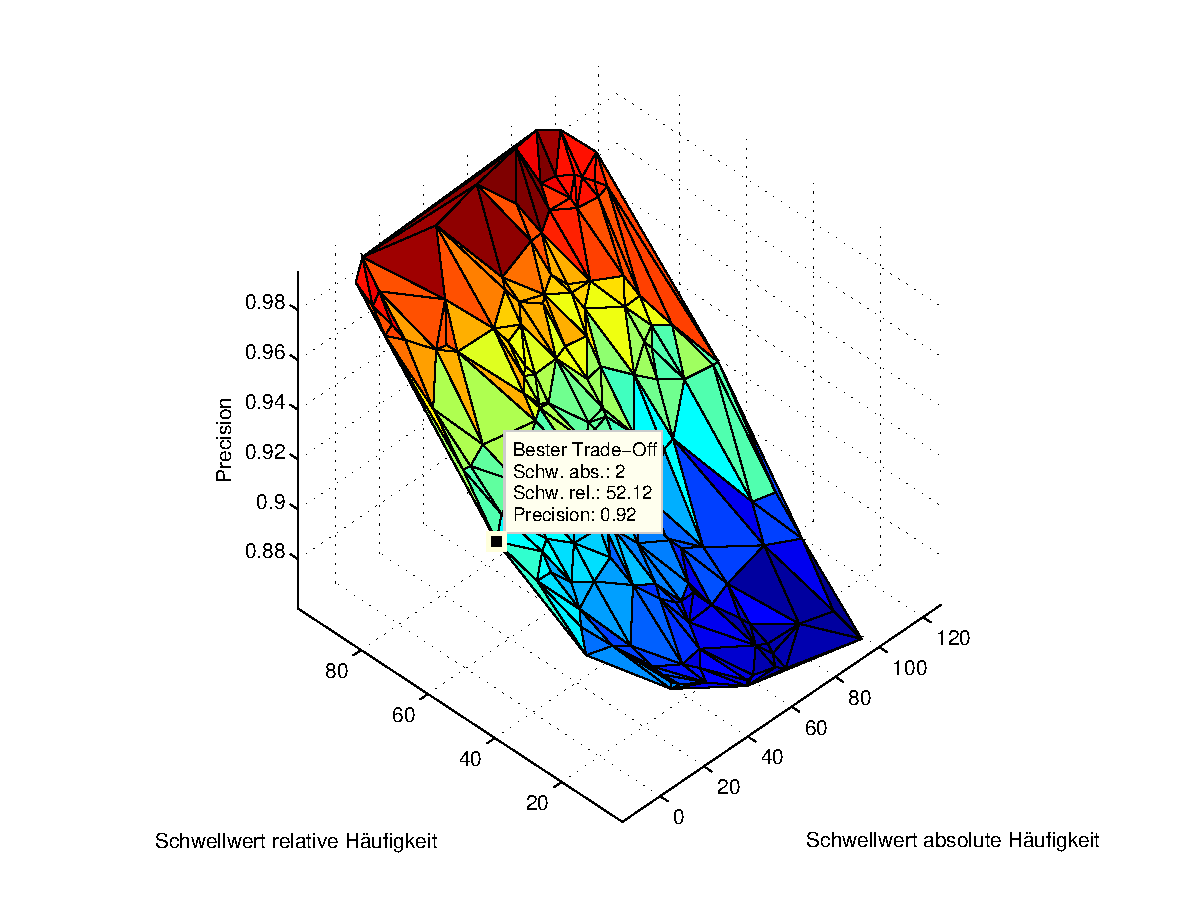
\includegraphics[width=.5\textwidth]{matlabPlot/coPrecision.eps}}
				       \\
				  \end{tabular}
				  
				  \caption{Precision Hierarchieebenen}
				  \label{img:precAll} 
				\end{figure}


				\newpage

				\begin{figure}[htb]
				\centering
				  \begin{tabular}{@{}ccc@{}}

				   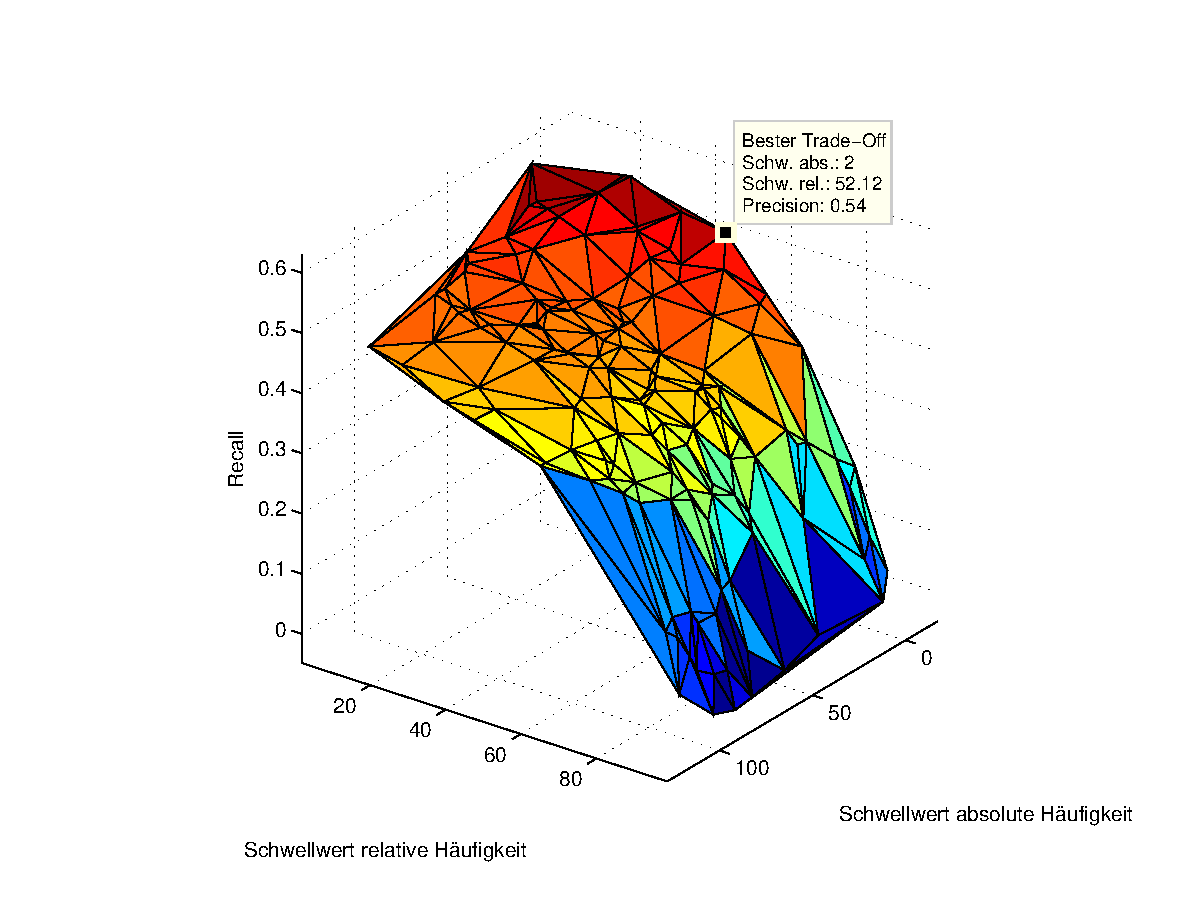
\includegraphics[width=.5\textwidth]{matlabPlot/adm1Recall.eps}	&
				    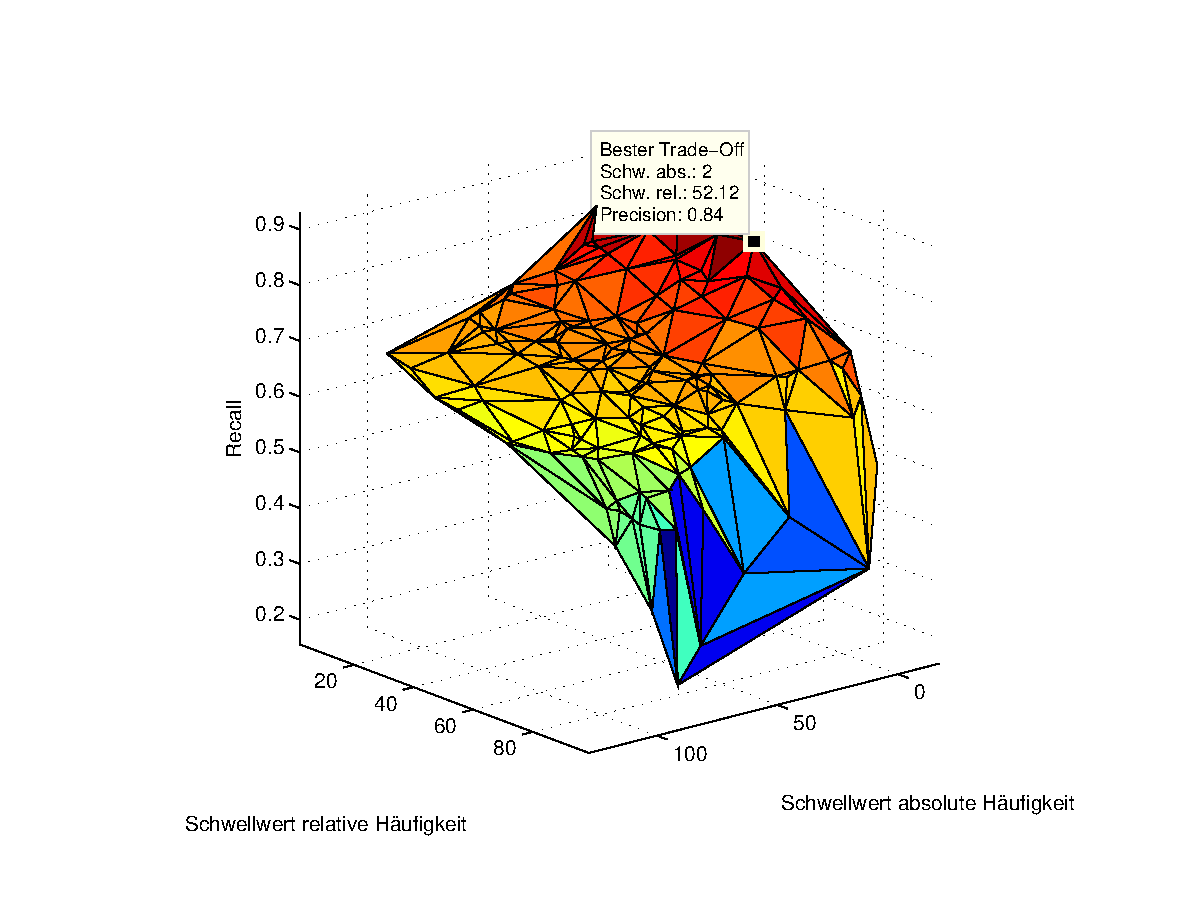
\includegraphics[width=.5\textwidth]{matlabPlot/coRecall.eps}  \\
				   \multicolumn{2}{c}{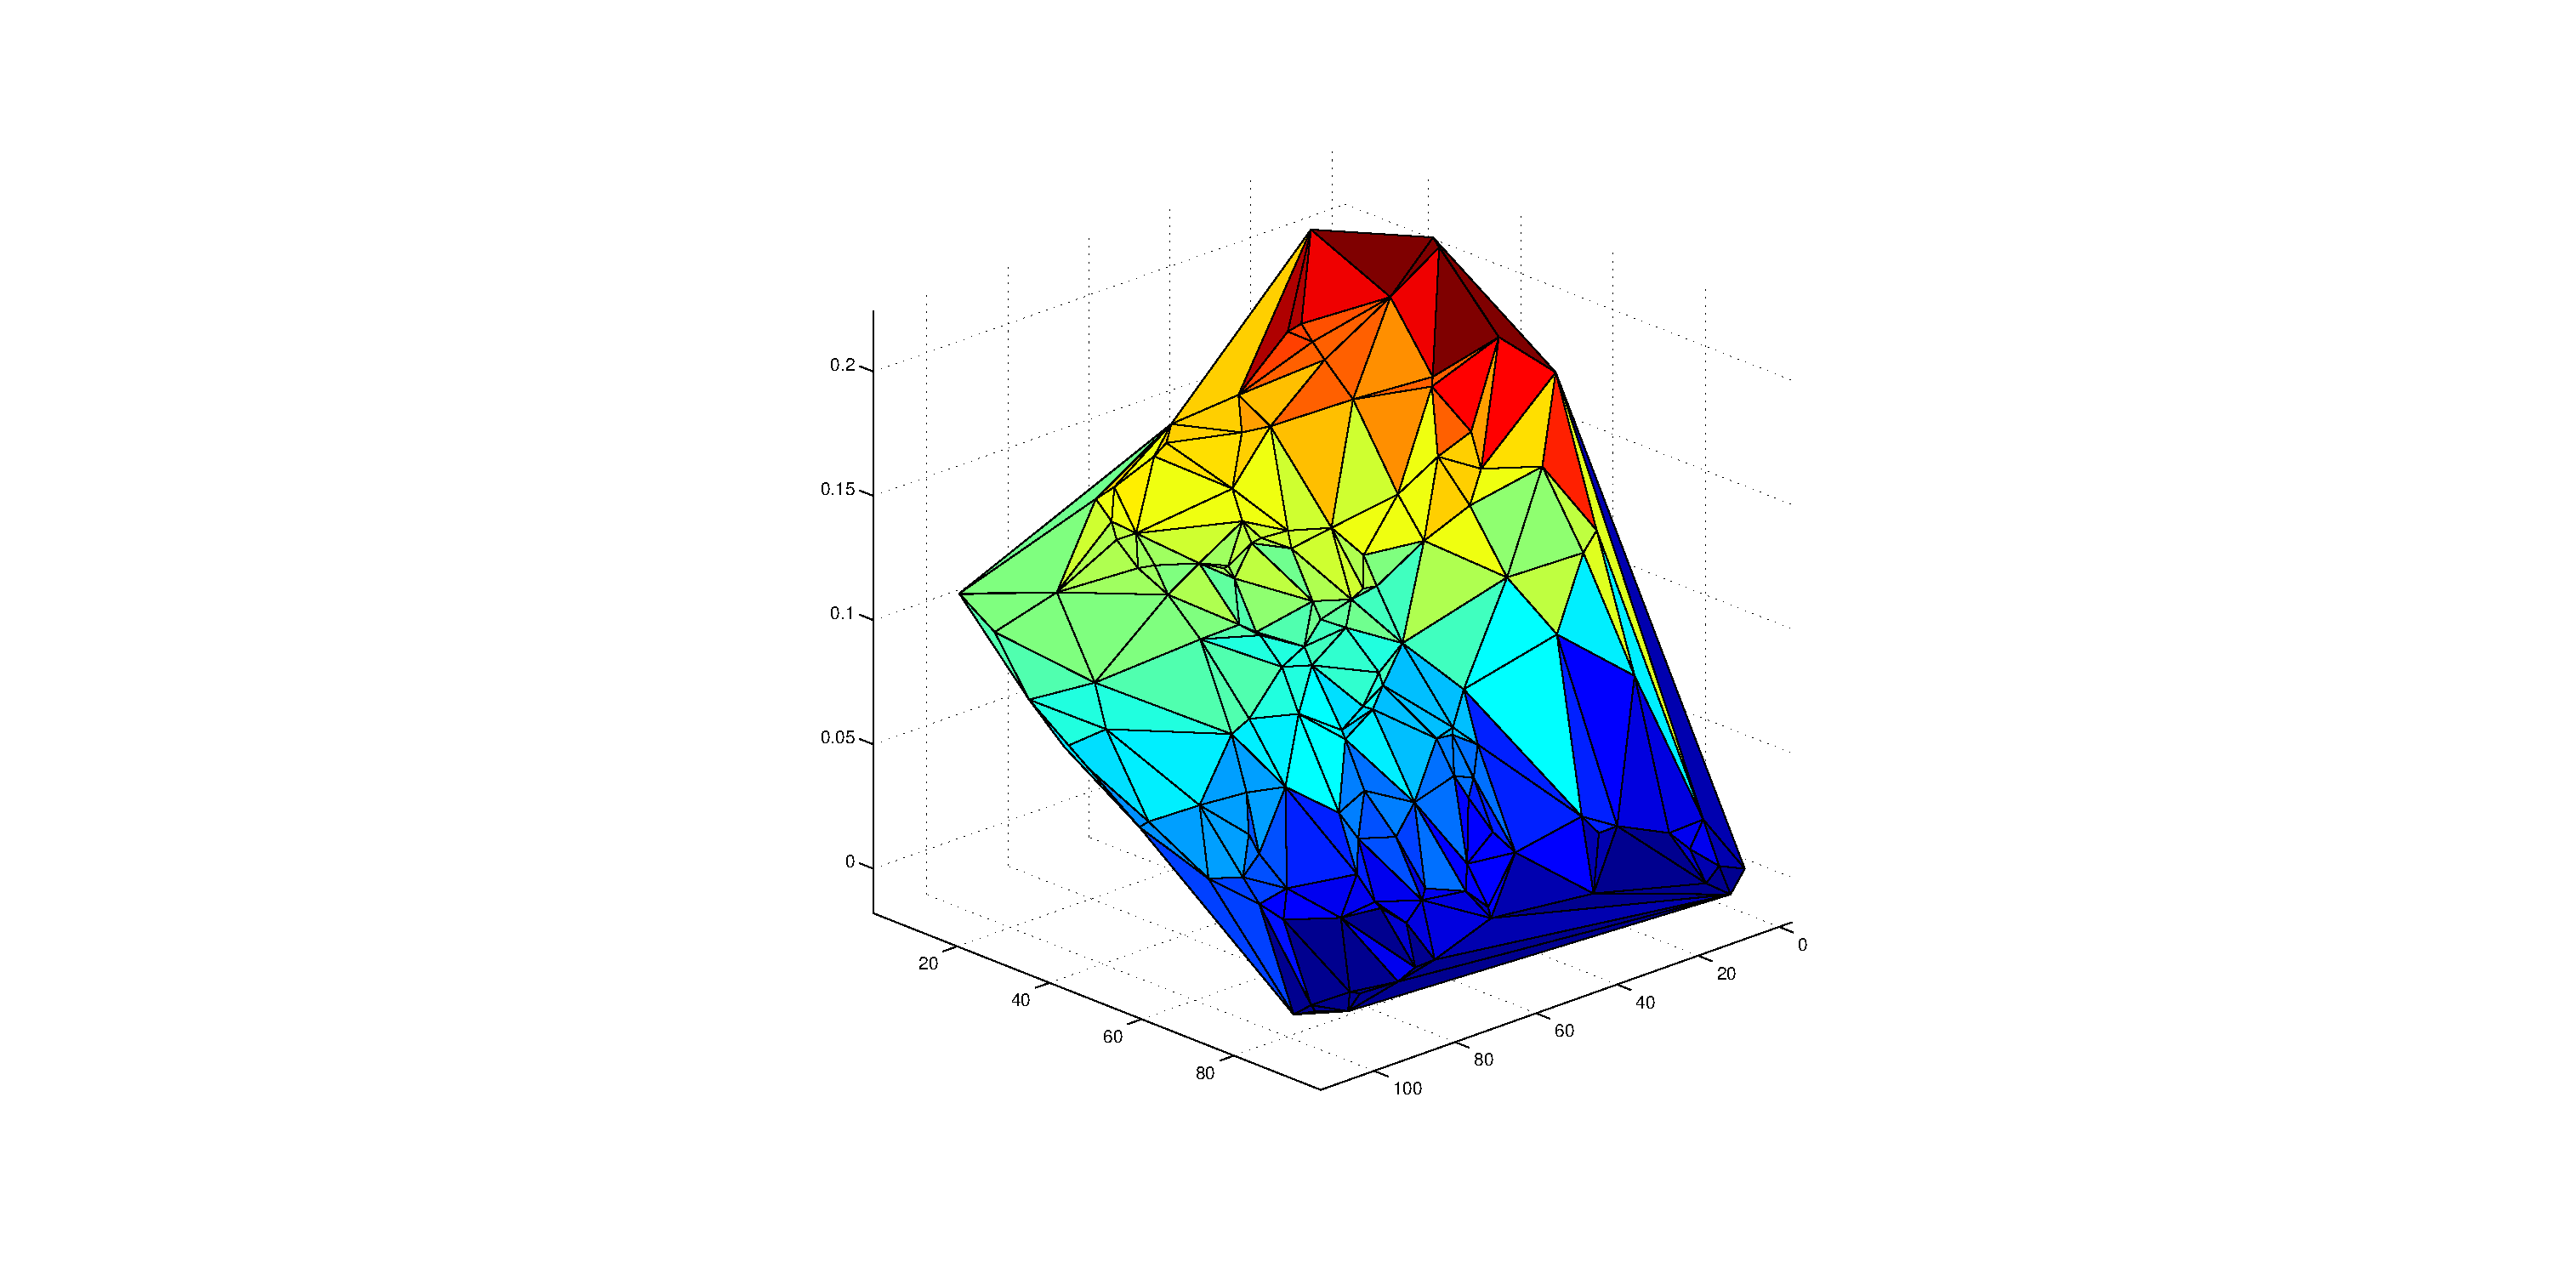
\includegraphics[width=.8\textwidth]{matlabPlot/adm2RecallNEW.eps}} \\
				  \end{tabular}

				  \caption{Recall Hierarchieebenen}
				  \label{img:recallAll} 
				\end{figure}


			Die besten Ergebnisse für die Hierarchieebenen sind in Tabelle \ref{tab:optAdm1Adm2Co} zusammengefasst.
			Auf Länderebene wird im besten Fall eine Precision von 0,99(99\%) erreicht.
			Dies bedeutet 99\% der Tweets konte das korrekte Land zugeordnet werden.
			Der Recall lag dagegen bei 24\%.

			Für den besten Trade-Off konnte der Recall auf 84\% erhöht werden, die Precision hat sich dabei nur unwesentlich auf 92\% reduziert. 
			Durch die Berechnung des besten Trade-Off konnten für die Verwaltungseinheiten erster und zweiter Orndung ähnliche Verbesserung erreicht werden.

			Für die Verwaltungseinheit erster Ordnung wird beim besten Trade-Off eine Precision von 80\% und ein Recall von 54\%, für die Verwaltungseinheit zweiter Ordnung eine Precision von 77\% und ein Recall von 12\% erreicht. 
			Das bedeutet besipielsweise für die Verwaltungseinheit zweiter Ordnung: Wenn eine Georeferenz zurückgeliefert wird ist diese mit einer Wahrscheinlichkeit von 77\% korrekt. 

				% Please add the following required packages to your document preamble:
			% \usepackage{multirow}
			\begin{table}[h]
			\centering
			\begin{tabular}{|l|l|l|l|l|l|}
			\hline
			                      &   & \multicolumn{1}{c|}{\begin{tabular}[c]{@{}c@{}}Schwellwert \\ relativ\end{tabular}} & \multicolumn{1}{c|}{\begin{tabular}[c]{@{}c@{}}Schwellwert\\ absolut\end{tabular}} & Precision     & Recall        \\ \hline \hline
			\multirow{3}{*}{Land} & 1 & 98.48                                                                      & 91                                                                        & \textbf{0.99} & 0.24          \\ \cline{2-6} 
			                      & 2 & 24.67                                                                      & 1                                                                         & 0.90          & \textbf{0.85} \\ \cline{2-6} 
			                      & 3 & 52.12                                                                      & 2                                                                         & \textbf{0.92} & \textbf{0.84} \\ \hline \hline
			\multirow{3}{*}{Adm1} & 4 & 98.48                                                                      & 91                                                                        & \textbf{0.97} & 0.001         \\ \cline{2-6} 
			                      & 5 & 26.84                                                                      & 2                                                                         & 0.71          & \textbf{0.58} \\ \cline{2-6} 
			                      & 6 & 52.12                                                                      & 2                                                                         & \textbf{0.80} & \textbf{0.54} \\ \hline \hline
			\multirow{3}{*}{Adm2} & 7 & 92.27                                                                      & 99                                                                        & \textbf{0.88} & 0.0007        \\ \cline{2-6} 
			                      & 8 & 24.67                                                                      & 1                                                                         & 0.48          & \textbf{0.21} \\ \cline{2-6} 
			                      & 9 & 65.39                                                                      & 7                                                                         & \textbf{0.77} & \textbf{0.12} \\ \hline
			\end{tabular}
			\caption{Beste Werte für Kennzahlen auf Adm1, Adm2 und Länderebene}
			\label{tab:optAdm1Adm2Co}
			\end{table}

			


		
		\subsection{Vergleich der besten Ergebnisse}

			In Tabelle \ref{tab:optAdm1Adm2Co} werden die besten Ergebnisse für Precision, Recall und Trade-Off betrachtet.
			In Zeile 1 wird der beste Wert für die Precision auf Länderebene dargestellt. 
			Dieser liegt bei 0,99. 
			Dies bedeutet 99\% der Tweets denen durch die Geolokalisierung ein Land zugeordnet werden konnte waren korrekt, dies ist ein optimaler Wert für die Precision.
			
			In Zeile 3 wird der beste Trade-Off auf Länderebene dargestellt.
			Bei einer Precision von 0,94 kann ein Recall von 0,84 erreicht werden. 
			Der Recall liegt damit lediglich 0,01 Zähler unter dem besten Recall aus Zeile 2.
			Die Precision wiederum liegt nur 7\% unter dem besten Wert aus Zeile 1. 
			
			Durch den optimalen Trade-Off erfahren Precision und Recall eine geringfügige Verschlechterung, insgesamt wird jedoch eine Verbesserung erzielt.
			Vor allem beim Vergleich des Recall Wertes in Zeile 1 (beste Precision) zu Zeile 3 (bester Trade-Off) ist eine Verbesserung von 60\% zu verzeichnen.
			Auf Kosten einer geringfügigen Verschlechterung der Precision wird der Recall um ein vielfaches verbessert.
			Die Änderung der Precision von Zeile 2 (bester Recall) zu Zeile 3 (bester Trade-Off) ist hingegen moderat. 
			Betrachtet man nun die Schwellwerte, fällt auf, dass in Zeile 2 (bester Recall) und 3 (bester Trade-Off) bei der absoluten Häufigkeit eine geringfügige Änderung von 1 Zähler vorliegt.
			Vergleicht man Zeile 1 (beste Precision) und 3 (bester Trade-Off) liegt eine sehr große Änderung von 89 Zählern bezüglich des Schwellwertes für die absolute Häufigkeit vor. 
			Dies legt die Vermutung nahe, dass die Veränderung der absoluten Häufigkeit eine immense Verbesserung des Recall zur Folge hat.
			Allerdings wird die Precision dadurch nur moderat verschlechtert. 

			Für die Verwaltungseinheit erster Ordnung (Adm1) ergibt sich ein ähnliches Bild. 
			Beim Vergleich zwischen den optimalen Werten von Precision und Recall zum optimalen Trade-Off ergibt sich eine Änderung von -17\% und -4\%.
			Die Ergebnisse der Verwaltungseinheit erster Ordnung sind insgesamt schlechter als dijenigen auf Länderebene. 

			


